\documentclass{sig-alternate}

\usepackage{url}
\usepackage{array}
\usepackage{multirow}

\newfont{\mycrnotice}{ptmr8t at 7pt}
\newfont{\myconfname}{ptmri8t at 7pt}
\let\crnotice\mycrnotice%
\let\confname\myconfname%

\permission{
Permission to make digital or hard copies of all or part of this work for personal or classroom use is granted without fee provided that copies are not made or distributed for profit or commercial advantage and that copies bear this notice and the full citation on the first page. Copyrights for components of this work owned by others than the author(s) must be honored. Abstracting with credit is permitted. To copy otherwise, or republish, to post on servers or to redistribute to lists, requires prior specific permission and/or a fee. Request permissions from Permissions@acm.org.}
\conferenceinfo{RecSys '15 Challenge,}{September 16-20 2015, Vienna, Austria \\
{\mycrnotice{Copyright is held by the owner/author(s). Publication rights licensed to ACM.}}}
\copyrightetc{ACM \the\acmcopyr}
\crdata{978-1-4503-3665-9/15/09 ...\$15.00\\
DOI: http://dx.doi.org/10.1145/2813448.2813510}

\clubpenalty=10000
\widowpenalty = 10000

\begin{document}

% --- Author Metadata here ---
%\conferenceinfo{RecSys}{'15 Vienna, Austria}
%\CopyrightYear{2007} % Allows default copyright year (20XX) to be over-ridden - IF NEED BE.
%\crdata{0-12345-67-8/90/01}  % Allows default copyright data (0-89791-88-6/97/05) to be over-ridden - IF NEED BE.
% --- End of Author Metadata ---

\title{RecSys Challenge 2015: ensemble learning with categorical features}
%\subtitle{[Challenge Solution]}

\numberofauthors{2}
\author{
% 1st. author
\alignauthor
Peter Romov\\
       \affaddr{Yandex Data Factory}\\
       \affaddr{Moscow, Russian Federation}\\
       \email{romovpa@yandex-team.ru}
% 2nd. author
\alignauthor
Evgeny Sokolov\\
       \affaddr{Yandex Data Factory}\\
       \affaddr{Moscow, Russian Federation}\\
       \email{esky@yandex-team.ru}
}

\date{\today}

\maketitle
\begin{abstract}
In this paper, we describe the winning approach for the~RecSys Challenge 2015.
Our key points are
(1) two-stage classification,
(2) massive usage of categorical features,
(3) strong classifiers built by gradient boosting and
(4) threshold optimization based directly on the competition score.
We describe our approach and discuss how it can be used
to build scalable personalization systems.
\end{abstract}

% A category with the (minimum) three required fields
\category{H.3.3}{Information Storage and Retrieval}{Information Filtering}
%A category including the fourth, optional field follows...
\category{I.2.6}{Artificial Intelligence}{Learning}

\keywords{Recommender systems, RecSys Challenge, Purchase prediction, Ensemble Learning, Categorical input data.}

\section{Introduction}

Web service personalization has become an area of growing research and commercial interest over the last years.
The major challenge here is to predict the user's intent given his online behavior history.
For example, an online retailer can attract a user by offering him some discount
on a specific item if the user's preference for this item is determined by his online profiles data and behavior history;
or an online travel agency can advertise a particular flight destination based on user's recent search details.
All such intents are usually detected by the means of machine learning.
Both users and businesses benefit from such personalization systems:
users receive more relevant offers and achieve their shopping goals faster;
businesses can get higher revenue and increased average basket size.

RecSys Challenge 2015~\cite{benshimon15recsys} is organized around a typical example of such problem.
We are given a history of user clicks during a browsing session at an e-commerce website,
and the goal is to predict the items the user will buy at the end
of this session.
Such data can be easily gathered by any e-commerce website,
so the challenge problem describes a common personalization case.

Our contribution is threefold:
(1) we construct high-quality predictive models for buyer sessions detection
and bought items prediction,
(2) we use those models to win the RecSys Challenge 2015,
(3) we show a way to simplify feature engineering process
with machine learning techniques in numerical and categorical feature spaces.

RecSys Challenge 2015 proposes an unconventional problem statement.
It requires to answer two questions:
\begin{enumerate}
    \item Which users are going to buy something?
    \item What items will users buy?
\end{enumerate}
Such statement motivated us to build two predictors,
one for each question.
The evaluation metric is quite difficult to optimize directly
for many reasons: the target space~(sets of items) is too complex,
the objective function is non-smooth, etc.
So we were bound to learn predictors with another, simpler objective~(namely log-loss).
However, we have found it feasible to find thresholds for predicted
probabilities that optimize the competition score directly.

We have found that lots of categorical features
can be extracted from the data that have
a good correlation with the user's buying intent.
However, we could not use common machine learning techniques
that can deal with categorical features
due to either their low capacity and inability to find
complex interactions~(e.g. linear classifiers)
or their inability to deal with such high-dimensional datasets~(e.g. XGBoost, Random Forest).
So, we ended up applying a special version of gradient boosting
that uses hash tables as weak learners and supports
categorical features with any number of levels.


\section{RecSys Challenge 2015: Problem Statement}
\label{sec:problem-statement}

The central task of the challenge is to predict what items the user will buy at the e-commerce website
given his click history.
In this section, we give more details on the data, describe the evaluation metric and
discuss some interesting properties of the challenge.

\subsection{Data Description}
Both training and test datasets comprise a set of user sessions~$S_\text{train}$,
$S_\text{test}$, where the size of the training set is approximately~$9.2 \cdot 10^6$
and of the test sets is approximately~$2.3\cdot 10^6$.
Each user session~$s$ from either training or test set
is represented as a click stream~$c(s) = (c_1(s), \dots, c_{n(s)}(s))$~---
a sequence of click events such that each click~$c_i(s)$ is described by:
\begin{itemize}
    \item timestamp~--- the time when the click occured;
    \item item ID~--- the unique identifier of the item;
    \item category~--- the category identifier of the item;
        the same item can belong to different categories in different click events.
\end{itemize}
The total number of item IDs and category IDs is~$54,287$ and~$347$ correspondingly.
Both training and test sets belong to an interval of 6 months.
The target function~$y(s)$ corresponds to the set of items that were bought in the session~$s$~\footnote{\small{
    Actually, the original data contains additional information
    for each buy event: timestamp, price and item quantity. However, we do not use any of it
    in the solution.
}}.
In other words, the target function gives some subset of the universal item set~$\mathbb{I}$
for each user session~$s$.
We are given sets of bought items~$y(s)$ for all sessions~$s$ the training set~$S_\text{train}$,
and are required to predict these sets for test sessions~$s \in S_\text{test}$.

\subsection{Evaluation Measure}
Denote by~$h(s)$ a hypothesis that predicts a set of bought items for any user session~$s$.
The score of this hypothesis is measured by the following formula:
\[
    Q(h, S_\text{test})
    =
    \sum_{\substack{s \in S_\text{test}: \\ |h(s)| > 0}}
    \Biggl(
        \frac{|S_\text{test}^b|}{|S_\text{test}|}
        (-1)^{\text{isEmpty}(y(s))} + J(y(s), h(s))
    \Biggr),
\]
where~$S_\text{test}^b$ is the set of all test sessions with at least one purchase event,
$J(A, B) = \frac{|A \cap B|}{|A \cup B|}$ is the Jaccard similarity measure.
It is easy to rewrite this expression as
\begin{equation}
\label{eq:score}
    Q(h, S_\text{test})
    =
    \underbrace{
        \frac{|S_\text{test}^b|}{|S_\text{test}|}
        (\text{TP} - \text{FP})
    }_{\text{purchase score}}
    +
    \underbrace{
        \sum_{s \in S_\text{test}}
            J(y(s), h(s))
        }_{\text{Jaccard score}},
\end{equation}
where~$\text{TP}$ is the number of sessions with~$|y(s)| > 0$ and~$|h(s)| > 0$~(i.e. true positives),
and~$\text{FP}$ is the number of sessions with~$|y(s)| = 0$ and~$|h(s)| > 0$~(i.e. false positives).
Now it is easy to see that the score consists of two parts.
The first one gives a reward for each correctly guessed session with buy events
and a penalty for each false alarm; the absolute values of penalty and reward are both equal
to~$\frac{|S_\text{test}^b|}{|S_\text{test}|}$.
The second part calculates the total similarity of predicted sets of bought items to the real sets.


\subsection{Purchase statistics}

It is interesting that sessions in training and test sets are not separated
in time, although it is considered a good practice for recommender problems
to predict future events based on a training set from the past.
This peculiarity allows us to use date-time features that appeared to be quite useful.

We define a~\textit{buying rate} as the fraction of buyer sessions
in some subset of sessions.
Figure~\ref{fig:buy-rate-time} shows how the buying rate changes in time.
It is obvious from the plots that visiting the e-commerce site during midday
leads to a purchase several times more often that in the night hours.
One will also make a purchase during his session with a higher probability on the weekend than on the working day.
Buying activity differs between all the days in the dataset,
e.g. there could be days of sales or holidays.
Another observation~(see Figure.~\ref{fig:buy-rate-unique-clicked}) is that a higher number of items clicked
during the session leads to a higher chance of a purchase.

Lots of information could be extracted from the data by considering
item identifiers and categories clicked during the session.
For example, we can find the item~$m(s)$ with the maximum number of clicks in each session~$s$.
In Figure~\ref{fig:buy-rate-unique-clicked} we show buying rates among sessions with specific
most clicked item~$m(s) = j$ for some popular item IDs~$j$.
It is easy to see that buying rates vary significantly among these IDs.

\begin{figure}
    \caption{Dynamics of the buying rate in time}
    \label{fig:buy-rate-time}
    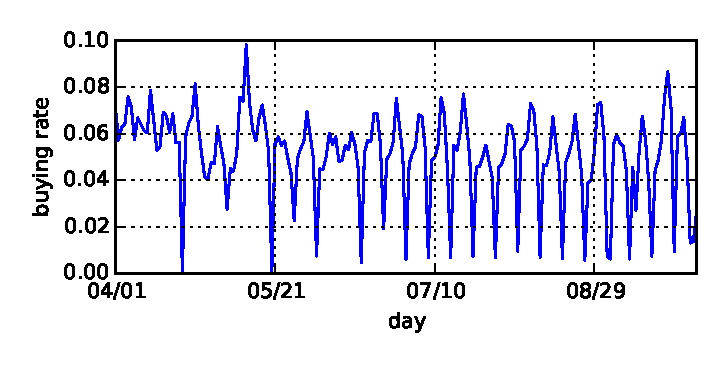
\includegraphics[width=8cm]{images/dataset_buyrate_day}
    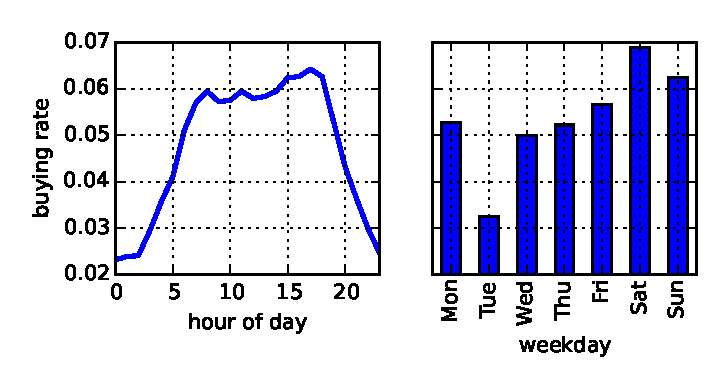
\includegraphics[width=8cm]{images/dataset_buyrate_hour_weekday}
\end{figure}

\begin{figure}
    \caption{Buying rate versus number of clicked items (left) and ID of the item with the maximum number of clicks in session (right)}
    \label{fig:buy-rate-unique-clicked}
    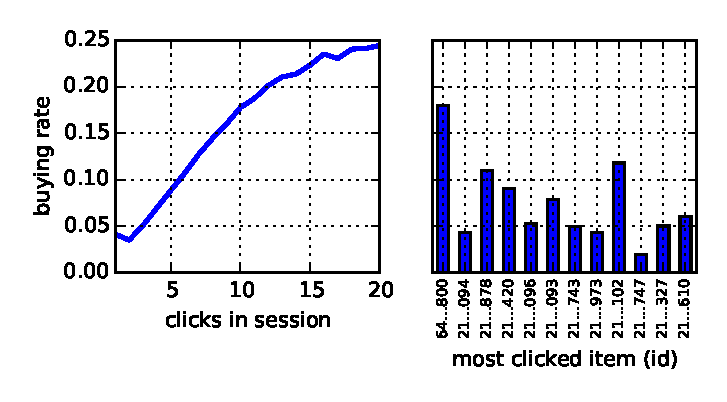
\includegraphics[width=8cm]{images/dataset_buyrate_clicks_items}
\end{figure}


\section{Solution Method}
\label{sec:solution}

\subsection{Outline}
Only 5.5\% of user sessions have at least one buy event,
so the problem is unbalanced: it appears to be important to be able
to predict whether the user will buy at least one item.
We have also noticed above that the evaluation measure consists of
two independent parts.
These considerations give us an idea to build a two-stage classifier:
at first, we predict whether the user will buy something,
and if the prediction is positive, then we predict what he will buy.
More precisely, we train \emph{purchase detection} and~\emph{purchased item detection} classifiers.
The purchase detection classifier~$h_p(s)$ predicts the outcome of the
function~$y_p(s) = \text{isNotEmpty}(y(s))$ and uses the entire training set in the
learning phase.
The item detection classifier~$h_i(s, j)$ approximates the
indicator function~$y_i(s, j) = I(j \in y(s))$ and uses only sessions with bought items
in the learning phase.

Of course, it would be wise to use classifiers that output probabilities rather
than binary predictions, because in this case we will be able to select thresholds that
directly optimize evaluation metric~\eqref{eq:score} instead of
the classifier's internal quality measure.
So, our final expression for the hypothesis can be written as
\begin{equation}
\label{eq:classifier}
    h(s)
    =
    \begin{cases}
        \emptyset & \mbox{if } h_p(s) < \alpha_p,\\
        \{j \in \mathbb{I}\ |\ h_i(s, j) > \alpha_i\} & \mbox{if } h_p(s) \geq \alpha_p.
    \end{cases}
\end{equation}

\subsection{Feature Extraction}
We have outlined two groups of features: one describes a session
and the other describes a session-item pair.
The purchase detection classifier uses only session features
and the item detection classifier uses both groups.
The full feature listing can be found in Table~\ref{tab:features};
for further details, please refer
to our code\footnote{\small{\url{https://github.com/romovpa/ydf-recsys2015-challenge}}}.
We give some comments on our feature extraction decisions below.

One could use sophisticated aggregations to extract numerical features that describe items and categories.
However, we utilize a simpler approach to add raw identifiers to the feature space instead.
The suitable learning method for such feature space will be discussed in the next section.

We have found it useful to calculate features based on what
is called~\emph{dwell time}~\cite{yi2014beyond} in information retrieval.
We define the~\emph{duration} for the click on the item~$j$
as the number of seconds between that click and the next click.
We have calculated features such as total duration of the item within the session,
total duration of the item's category, etc.

\begin{table*}
    \caption{List of features used in models.}
    \label{tab:features}
    \medskip
    \centering
    \begin{tabular}{|m{2cm}|p{12cm}|m{2.5cm}|}
        \hline
        \bfseries{Group} & \bfseries{Feature Description} & \bfseries{Number/Type} \\
        \hline
        \hline % session
        \multirow{7}{*}{\parbox{2cm}{\centering Session features}}
            & Numerical time features of the start/end of the session~(month, day, hour, minute, second, etc.)
            & 2 $\times$ 7 Num \\ \cline{2-3}
        & Categorical time features of the start/end of the session~(month, day, month-day, month-day-hour, hour, minute, weekday)
            & 2 $\times$ 7 Categ \\ \cline{2-3}
        & Length of the session in seconds & 1 Num \\ \cline{2-3}
        & Number of clicks, unique items, categories and item-category pairs in the session & 4 Num \\ \cline{2-3}
        & Top 10 items and top 5 categories by the number of clicks in the session & 15 Categ \\ \cline{2-3}
        & IDs of the first/last item clicked at least $k=1,2\dots,6$ times in the session & 12 Categ \\ \cline{2-3}
        & Vector of click numbers and total durations for 100 items and 50 categories that were the most popular in the whole training set
            & 150 $\times$ 2 Num \\ \hline
        \hline % session-item
        \multirow{8}{*}{\parbox{2cm}{\centering Paired session-item features}}
            & Item ID & 1 Categ \\ \cline{2-3}
        & Total and relative number of clicks in the session for the given item & 2 Num \\ \cline{2-3}
        & Numerical time features of the first/last click on the item~(month, day, hour, minute, second, etc.)
            & 2 $\times$ 7 Num \\ \cline{2-3}
        & Categorical time features of the first/last click on the item~(month, day, month-day, month-day-hour, hour, minute, weekday)
            & 2 $\times$ 7 Categ \\ \cline{2-3}
        & Number of seconds between the first and the last click on the item & 1 Num \\ \cline{2-3}
        & Total duration of the clicks on the item in the session and of all item's categories seen in the session & 2 Num \\ \cline{2-3}
        & Number of unique categories seen in the session for a given item & 1 Num \\
        \hline
    \end{tabular}
\end{table*}

\begin{figure}
    \caption{Item detection threshold~(above) and purchase detection threshold~(below) quality on the validation set.}
    \label{fig:thresh}
    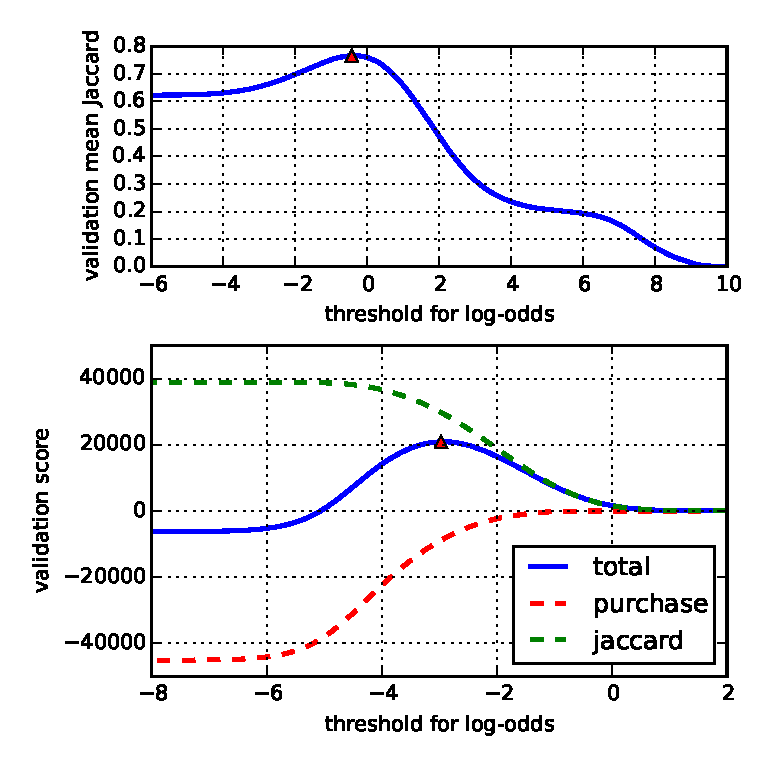
\includegraphics[width=8cm]{images/thresholds}
\end{figure}

\subsection{Classification Method}
\label{sec:classification}

The main challenge of our dataset is that it contains
dozens of categorical features with tens of thousands levels.
Popular ensembling libraries~(e.g. XGBoost, \texttt{ensemble} in sklearn, \texttt{gbm} in R)
do not support categorical features directly
and require them first to be transformed to real-valued features, e.g. by one-hot encoding.
However, one-hot encoding of our dataset would lead to the unfeasible number of features.
To overcome this problem, we relied on Yandex' proprietary machine learning
tool called MatrixNet~\cite{mxnetslides}.
It is an implementation of gradient boosting~\cite{friedman00greedyfunction}
over oblivious decision trees~\cite{kohavi95odt} with careful leaf values weighting based
on their variance.
To extend this approach to categorical features, MatrixNet uses hash tables as base learners.
One hash table corresponds to a small subset of features
and contains predictions for all value combinations of these features seen on a training set.
MatrixNet also builds SVD-like low-rank approximations%~\cite{koren2009matrix}
of hash tables for the case
it will encounter new feature value combinations in the test set~(for example, suppose that a table
contains features ``User ID'' and ``Movie ID'', and we want to predict
a user rating for a film the user had not seen before).

Friedman~\cite{friedman00greedyfunction} proposed to select features
for decision trees based on MSE gain.
It works quite well for real-valued features, but the presence of categorical features
in the training set can lead to more complex hash tables and severe overfitting due to the nature of MSE gain.
We cope with this problem in MatrixNet by using a generalization bound-based criterion~(e.g.~\cite{tolstikhin13pacbayes})
for feature selection.

Since both learning tasks in our solution schema are binary classification tasks,
we have selected binary log-likelihood as a loss function.
To improve convergence for this function, MatrixNet performs an additional optimization.
When the hash table is built and predictions in each record
are calculated based on MSE~(recall that weak learners are always trained using MSE criterion
regardless the actual objective function~\cite{friedman00greedyfunction}),
MatrixNet performs univariate optimization in each hash table record separately by gradient descent over log-likelihood.
We have trained classification models in distributed mode on Yandex's cluster of 150 machines.
It took about 12 hours to train both models, and their size turned out to be about 60 gigabytes.
The final prediction for the test set was generated in 10 minutes in one thread on the single machine,
what corresponds to a prediction speed of approximately 4000 sessions per second.

\subsection{Threshold Optimization}
We have selected~90\% of the training set for the learning purposes
and~10\% for the validation.
The purchase and item detection classifiers~$h_p(s)$ and~$h_i(s, j)$
were trained by MatrixNet on the learning part with the optimal
number of weak learners selected on the validation set.
Then we used the validation set to find the best thresholds
for purchase detection~($\alpha_p \approx -2.97$) and item detection~($\alpha_i \approx -0.43$) classifiers.

To make the final predictions on the test set we first maximize the mean Jaccard similarity
for validation samples by choosing the optimal item threshold $\alpha_i$.
Then we fix $\alpha_i$ and optimize the competition score~\eqref{eq:score}
by choosing the optimal purchase threshold $\alpha_p$.
The first optimization is performed by using a standard univariate optimization method,
the objective function is shown in Figure~\ref{fig:thresh}~(above).
The purchase threshold can be found simply by a single pass through the sessions
in the validation set ordered by the predicted probability,
the objective function~(competition score) is shown in Figure~\ref{fig:thresh}~(below).
The behavior of both summands from the competition score~\eqref{eq:score}
is also shown in that Figure: the Jaccard score monotonically decreases
and the purchase score monotonically increases as we increase the threshold for
purchase probability.
One can say that purchase threshold optimization is concerned with finding
the optimal balance between these two scores.

Although we have optimized a quite specific measure,
the purchase detection classifier achieves a high AUC value of~$0.85$
on the validation set.
It has 16\% precision and 77\% recall for optimal thresholds~$\alpha_p$ and~$\alpha_i$,
so competition measure~\eqref{eq:score}
tends to maximize recall rather than precision.
The item detection classifier achieves mean Jaccard measure of~$0.765$.


\section{Conclusions}
Our solution has several key points:
\begin{enumerate}
    \item Feature extraction: we have calculated about 400 features concerned with clicked items
        and categories, item popularity, click duration.
    \item Two-staged classification: at first we predict whether the user will buy something,
        and if yes, we predict the exact subset of items he will buy.
    \item Threshold optimization: we select the prediction threshold that optimizes the competition score directly.
    \item Classification model: we use Yandex' implementation of gradient boosting
        that uses hash tables as weak learners and easily deals with categorical features.
        The model can generate about 4000 predictions per single thread per second
        which is enough for building a scalable personalization service.
\end{enumerate}

Our prediction model has a good quality and scalability and can be used
for online personalization purposes in a variety of cases that serve the same goal~---
increasing customer's engagement and overall satisfaction.
The achieved quality of purchase and item detection allows providing highly personalized
product offers, ads, shopping recommendations, or entire sales strategies.

\section{Acknowledgments}
This work was conducted at Yandex Data Factory\footnote{\small{\url{https://yandexdatafactory.com/}}}
as part of the ``Next best offer'' recommender service project.

%% Bibliography
\bibliographystyle{abbrv}
\bibliography{sigproc}

%APPENDICES are optional
%\balancecolumns
%\appendix

\end{document}
